\documentclass{article}
\usepackage[utf8]{inputenc}

\title{Tarea 1 modelos probabilísticos aplicados}
\author{Romulo Enrique Troncoso Pacheco }
\date{Septiembre  2020}

\usepackage{natbib}
\usepackage{graphicx}

\begin{document}

\maketitle

\section{Introducción}
Los datos que se tomaron de la pagina del INEGI\citep{INEGI} en el apartado de agricultura fueron sobre Superficie cultivada y producción de cultivos anuales y perennes según tipo de agricultura por cultivo con representatividad en la muestra los cuales feuron recolectados en las fechas de 2016 a septiembre de 2017.
\newline
Nombre del archivo original: 'ena17agri01.xlsx'.
\newline
Con estos datos se pretende realizar una practica de graficación de datos en el lenguaje de programación R.
\section{Interpretación}
A este cúmulo de datos se le puede interpretar de tal manera en donde se le pueden hacer graficas de tipo circular , grafica de barras y grafica de puntos  ya que por ser solo un punto relacionado con una etiqueta. 
\newline
Estos datos nos muestran la producción de productos agrícolas a lo largo de un tiempo determinado (octubre de 2016 a septiembre de 2017) basándose en tres datos relevantes:
\begin{itemize}
    \item Hectáreas sembradas.
    \item Hectáreas cosechadas.
    \item Toneladas recolectadas.
\end{itemize} 
Estas agrupadas  en dos especies
\begin{itemize}
    \item Cielo abierto.
    \item Invernadero.
\end{itemize} 
\section{Riesgos}
\begin{itemize}
    \item Los valores entre los campos sean desproporcionados evitando ver la grafica de mejor manera.
    \item Al contar con demasiados cultivos en las graficas se podrá presentar un overlap con los nombres de los cultivos.
\end{itemize}   
    
\section{Objetivos}
\begin{itemize}
  \item Graficar los datos a cielo abierto en relación a hectáreas sembradas,hectáreas cosechadas y producción en toneladas por tipo de cultivo
  \item Graficar los datos en invernadero en relación a hectáreas sembradas y  producción en toneladas por tipo de cultivo
  \item Graficar la producción total en relación al cultivo y toneladas cosechadas
  \item Calcular las hectáreas sembradas tanto en aire libre e invernadero
  \item Calcular  el porcentaje de hectáreas sembradas conforme al cultivo
  \item Graficar en forma circular y en forma de barra los porcentajes
  \item Calcular las hectáreas perdidas en base a las hectáreas sembradas y las hectáreas cosechadas  por cultivo
  \item Graficar en forma circular y en forma de barra las hectáreas perdidas 
\end{itemize}

\section{Prerrequisitos}
\subsection{Preprocesamiento}
Se crearon dos archivos en formato csv ya que el archivo que se descarga de la pagina de INEGI\citep{INEGI} contiene datos basura que afectan a la manipulación del mismo, en los archivos csv se conservo el orden de los datos unicamente separando los datos de cielo abierto y de invernadero.\newline
Nombre de los formatos:
\begin{itemize}
    \item 'Cielo abierto.csv'
    \item 'invernadero.csv'
\end{itemize}

\subsection{Paqueteria y versionado}
Para la generación de las graficas se utilizo el lenguaje de programación R en su versión 4.0.2\citep{LR} en conjunto con el editor visual studio code\citep{VS-code}. \newline
Internamente se utilizaron las siguientes librerías:
\subsubsection{readr}
Descripción:\newline
El objetivo de 'readr' es proporcionar una forma rápida y sencilla de leer datos rectangulares (como 'csv', 'tsv' y 'fwf').\newline
Versión:\newline
1.3.1\newline
Repositorio:\newline
https://cran.r-project.org/web/packages/readr/index.html

\subsubsection{plotrix}
Descripción:\newline
Contiene una gran cantidad de gráficos, diversas funciones de etiquetado, eje y escala de color.\newline
Versión:\newline
3.7.8\newline
Repositorio:\newline
https://cran.r-project.org/web/packages/plotrix/index.html


\section{Salida}

\begin{figure}[ht]
\centering
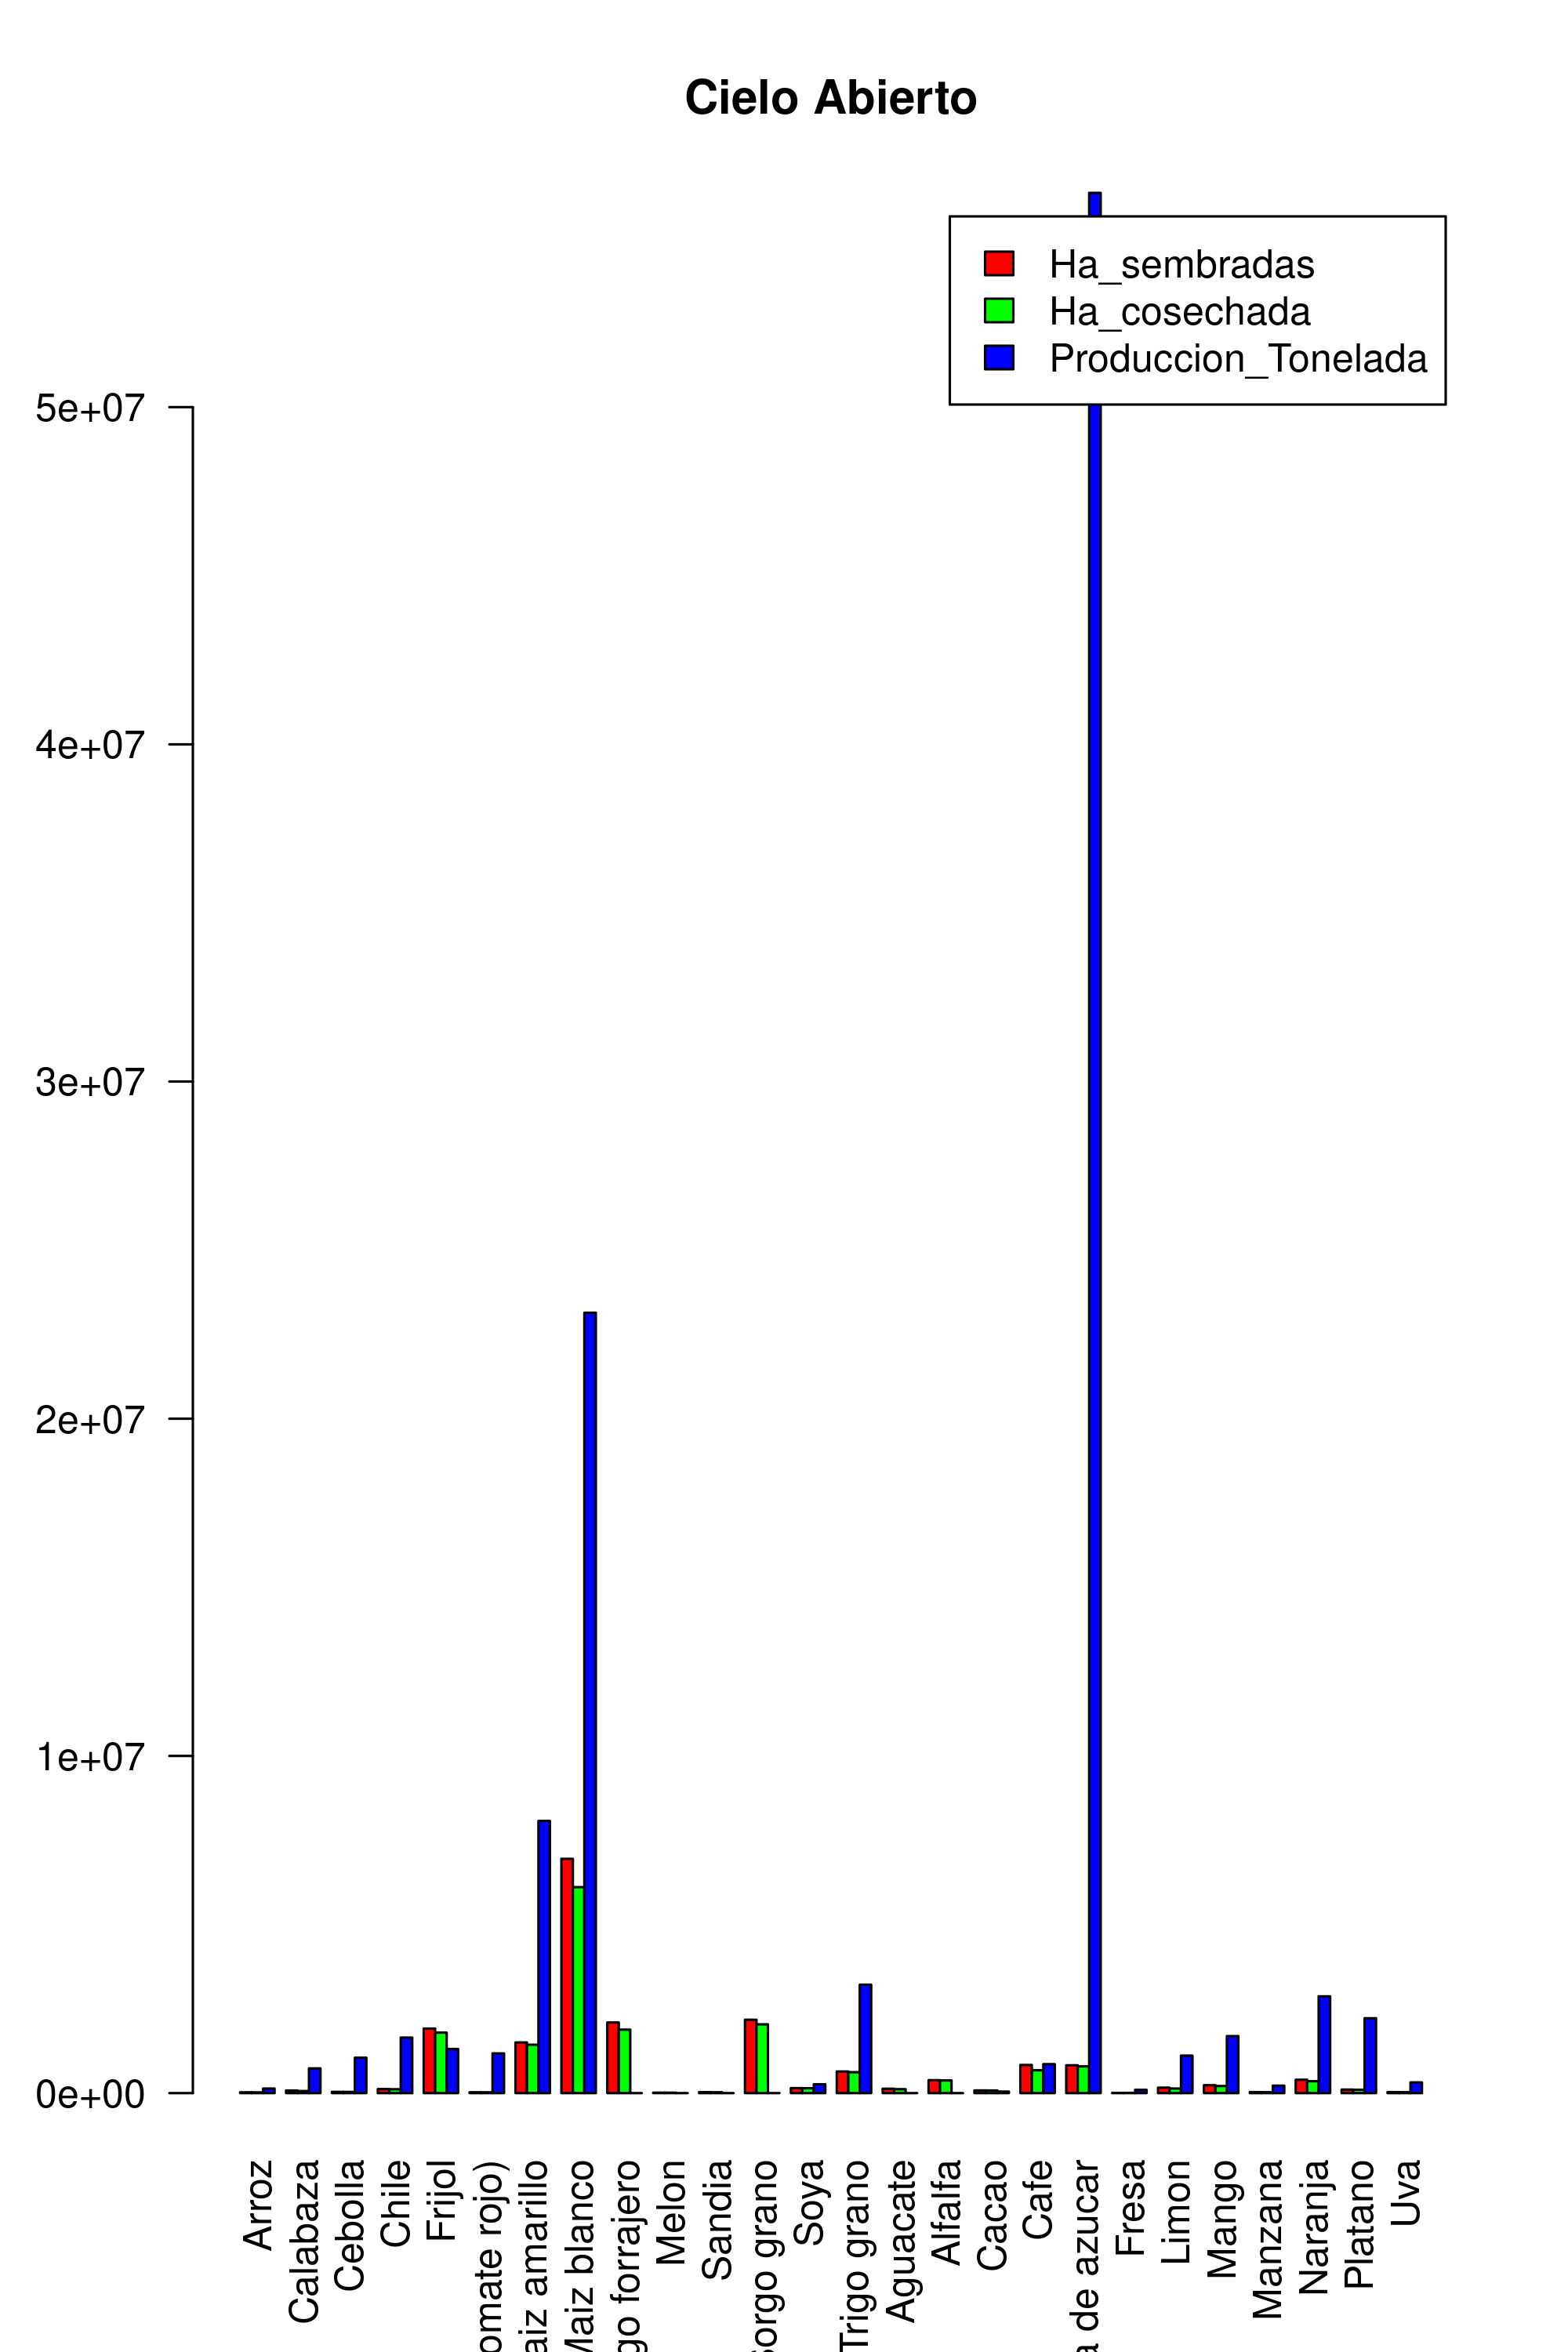
\includegraphics[scale=.5]{Tablas_Cielo_Abierto.png}
\caption{Relación hectáreas sembradas,hectáreas cosechadas y producción en toneladas por tipo de cultivo.}
\label{fig:Cielo_abierto}
\end{figure}
\begin{figure}[ht]
\centering
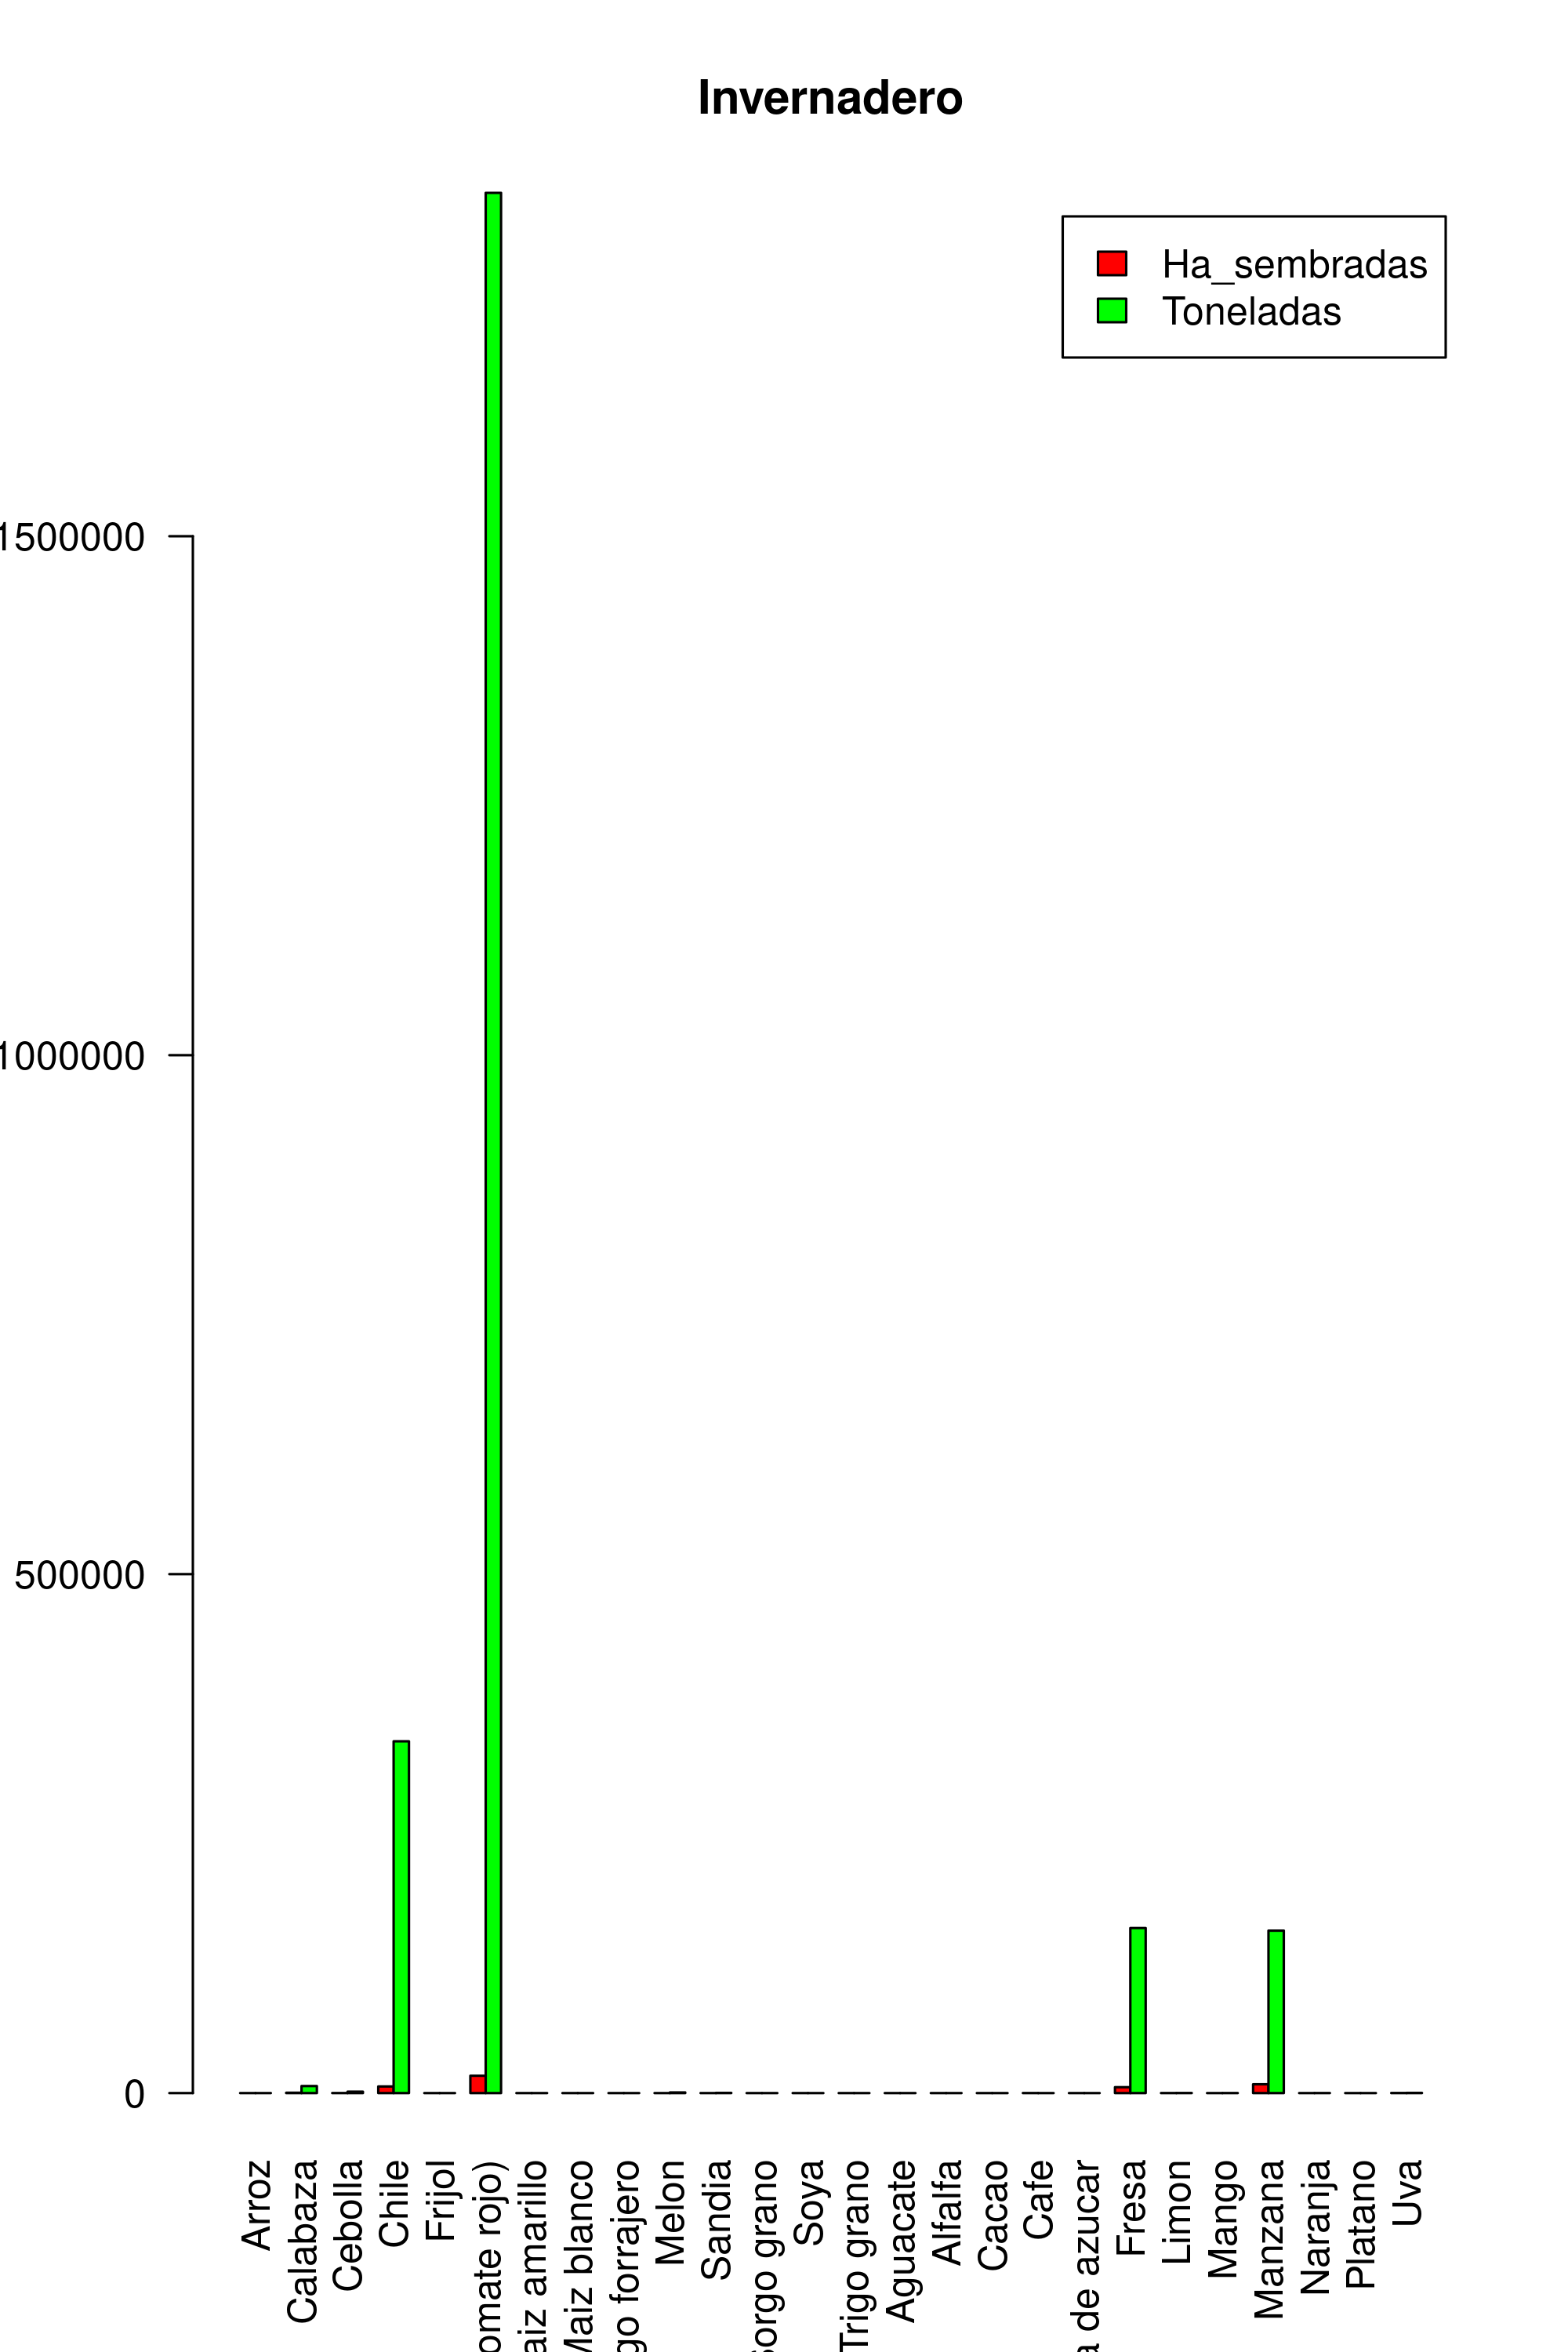
\includegraphics[scale=.5]{Tablas_invernadero.png}
\caption{Relación hectáreas sembradas y producción en toneladas por tipo de cultivo.}
\label{fig:invernadero}
\end{figure}
\begin{figure}[ht]
\centering
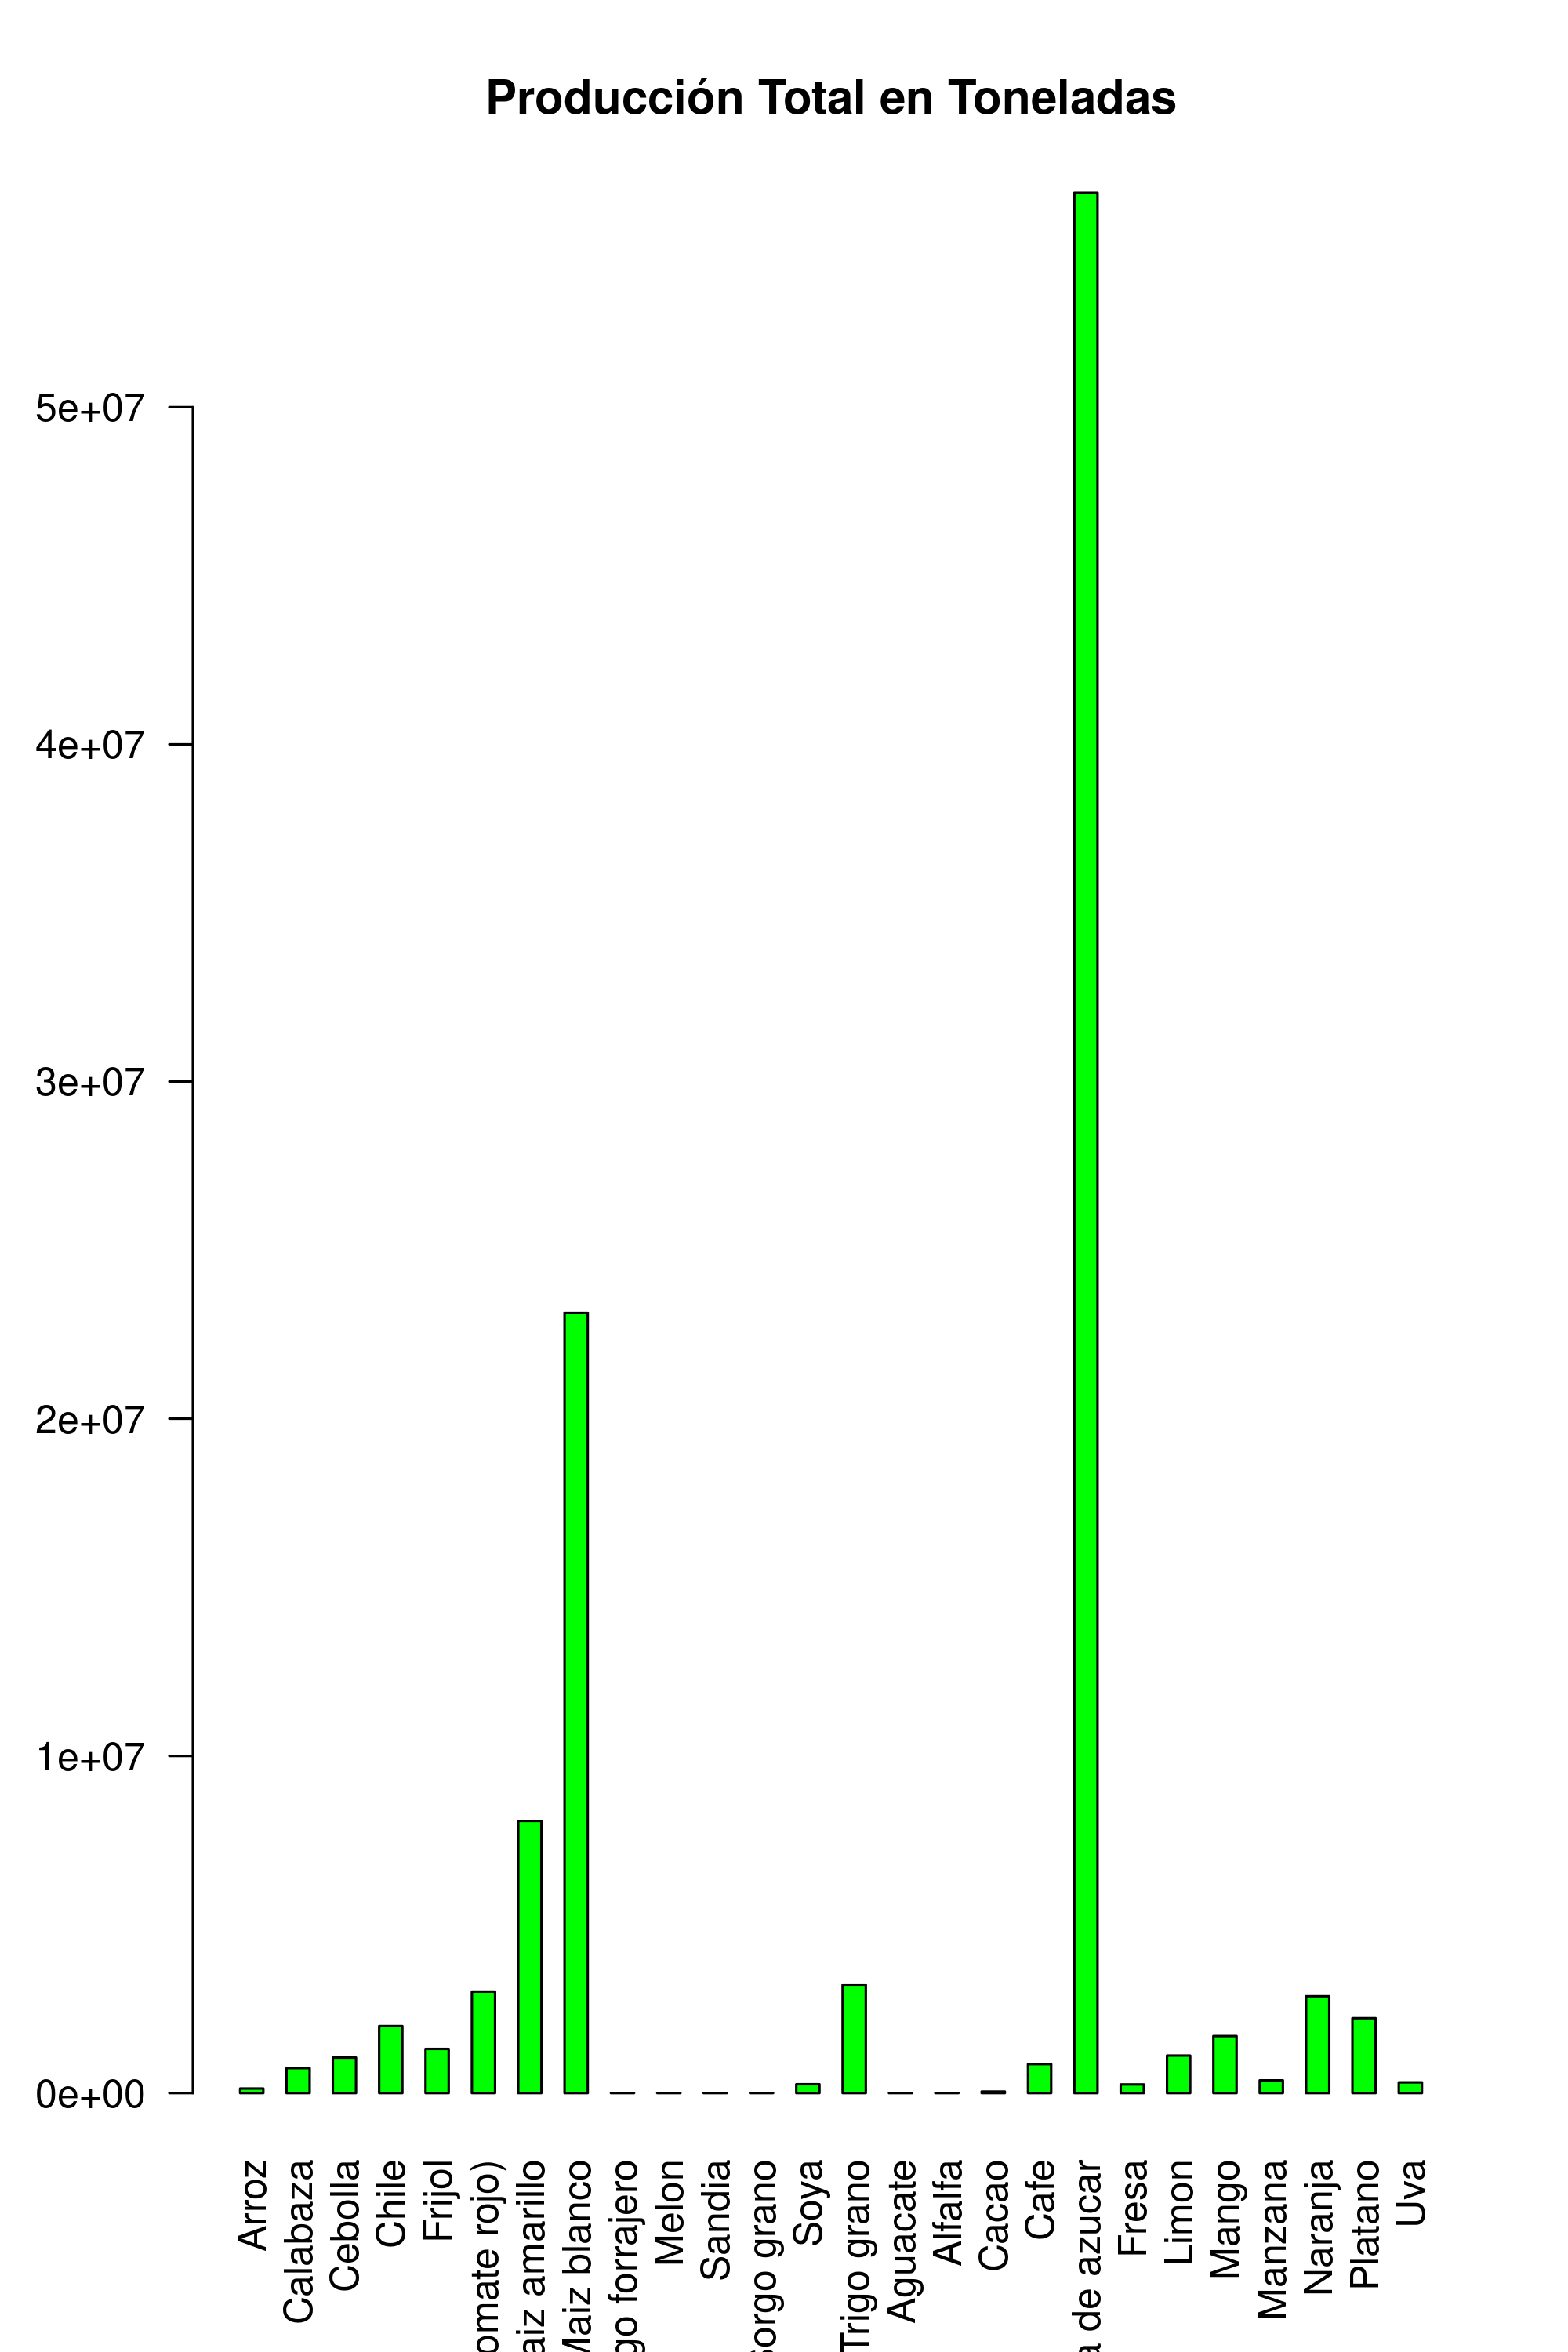
\includegraphics[scale=.5]{Tablas_Produccion_Total.png}
\caption{Muestra la cantidad de toneladas cosechadas por cultivo}
\label{fig:produccion_total}
\end{figure}
\begin{figure}[ht]
\centering
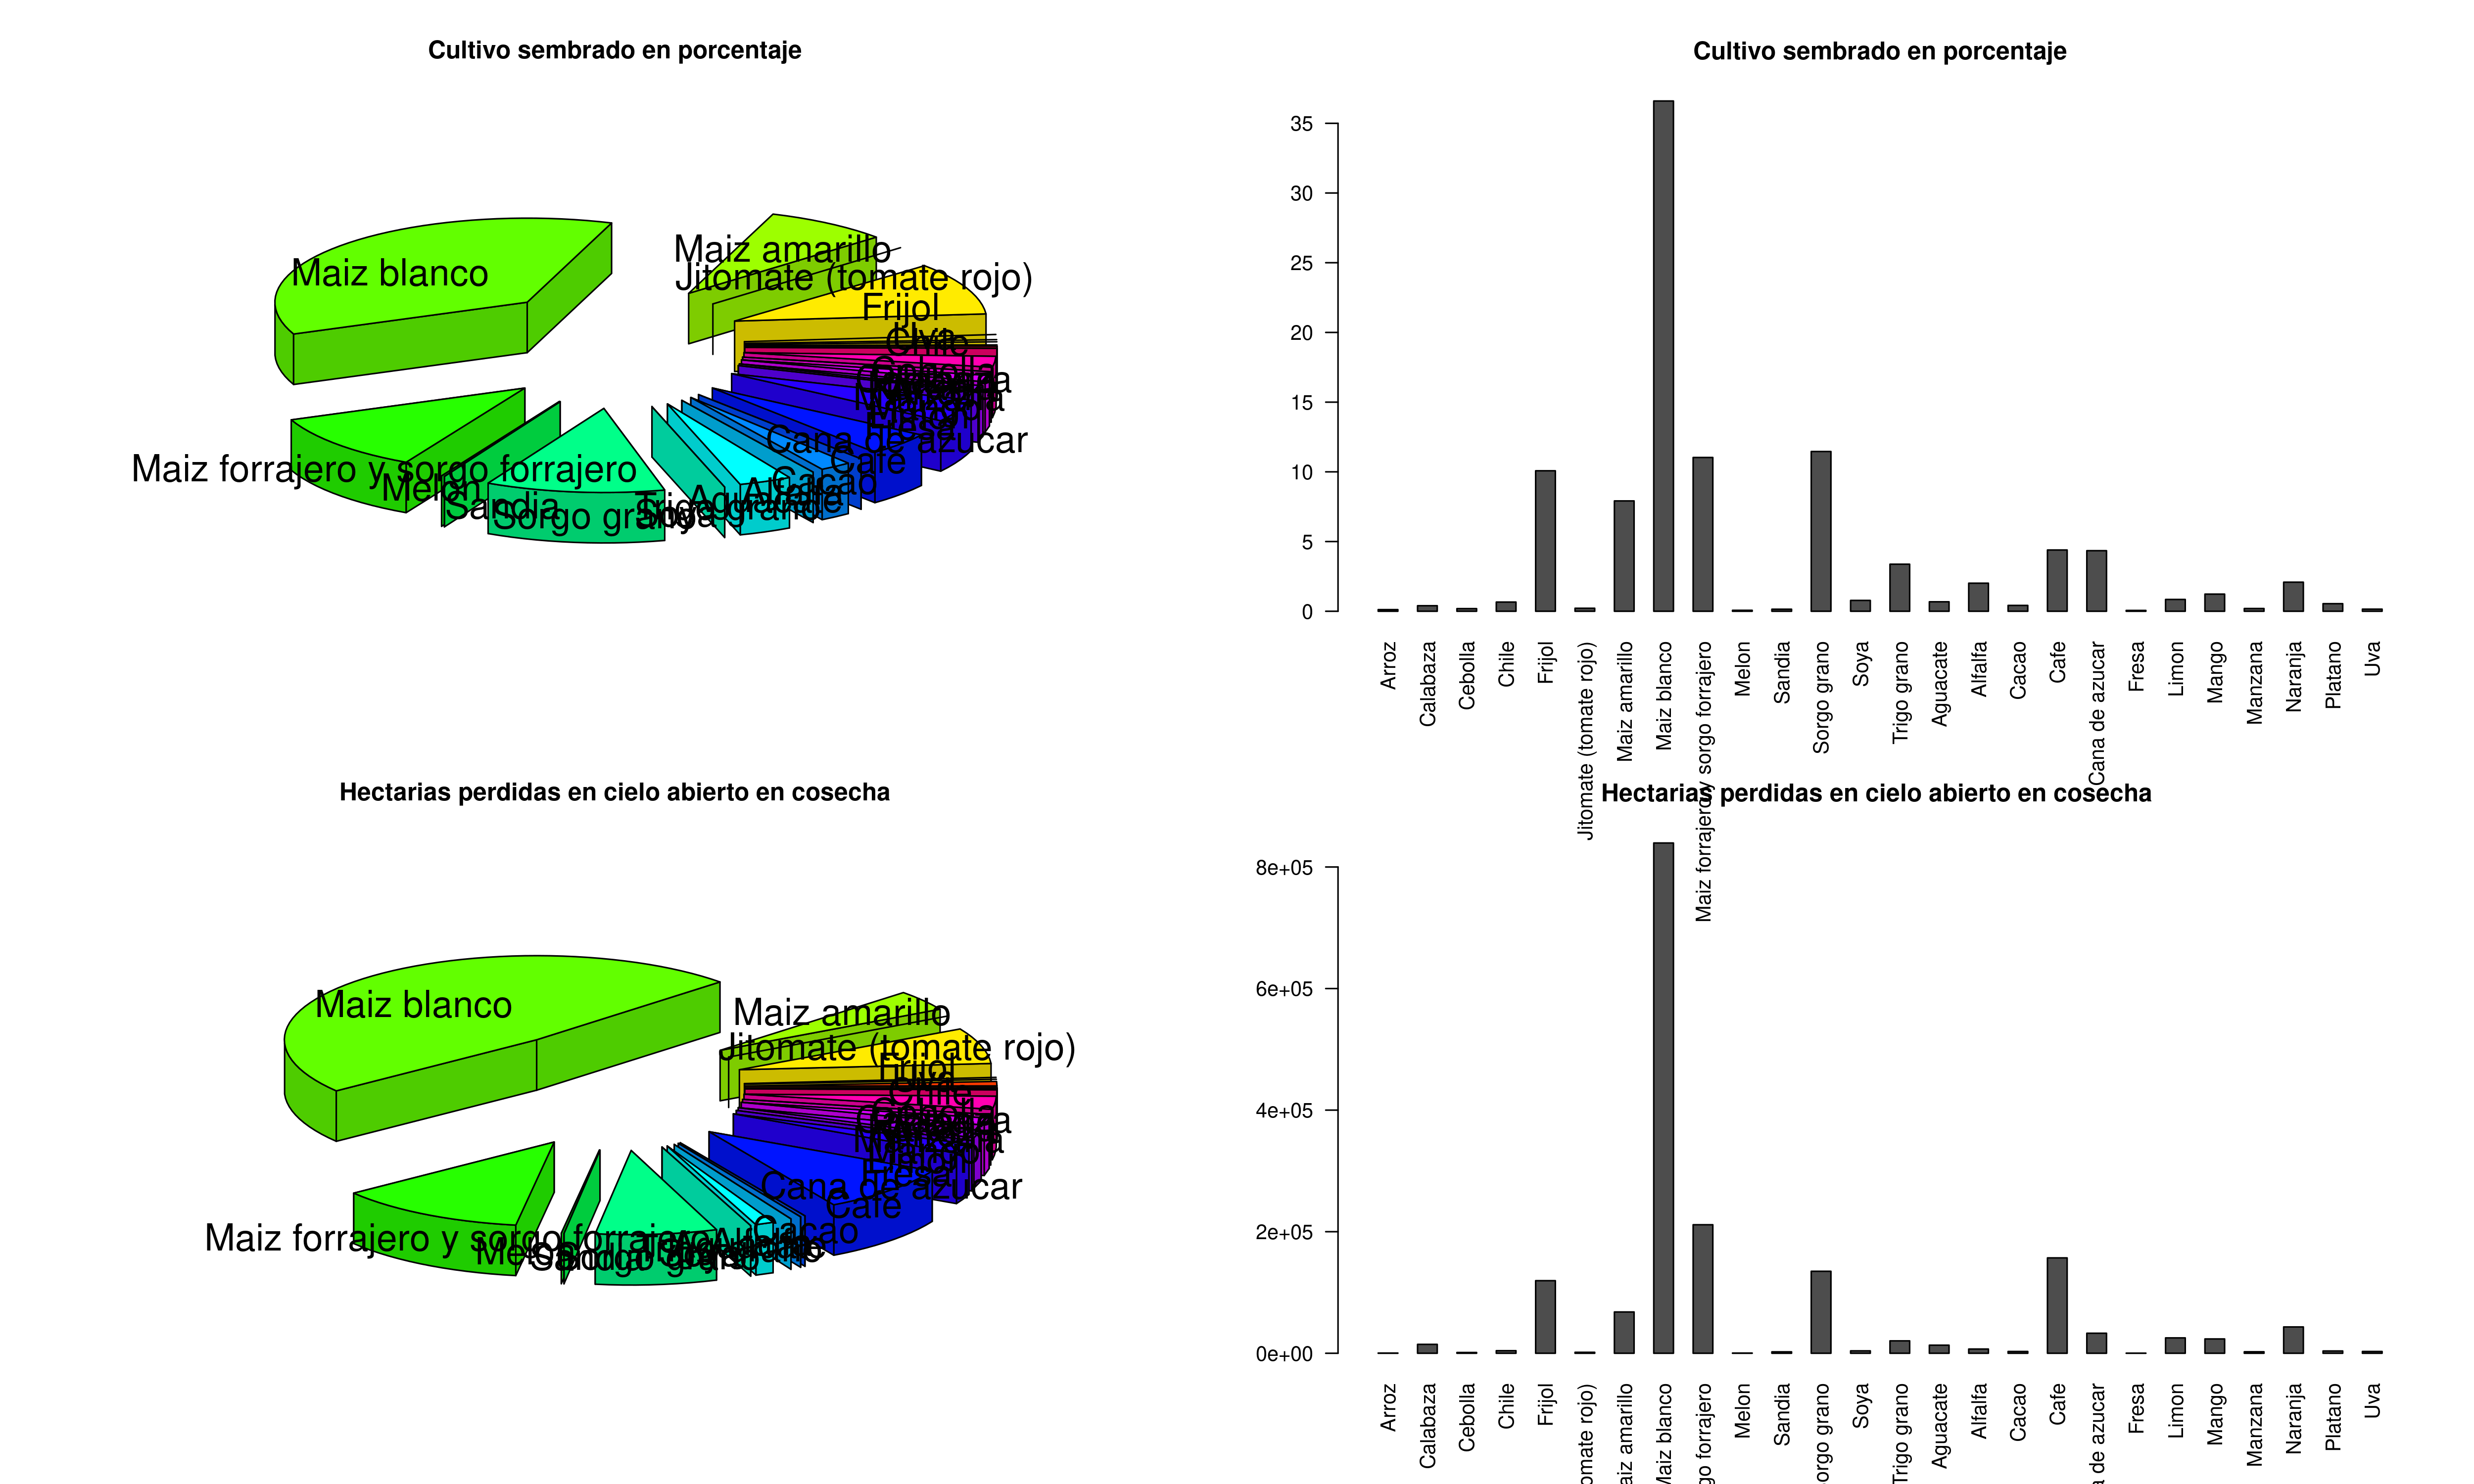
\includegraphics[scale=.4]{Tablas_Comparativos.png}
\caption{Muestra del porcentaje de hectáreas cosechadas por cultivo y perdida de hectáreas en forma de pastel y barras}
\label{fig:produccion_total}
\end{figure}


\clearpage
\bibliography{references}
\bibliographystyle{plain}
\end{document}
